%%%%%%%%%%%%%%%%%%%%%%%%%%%%%%%%%%%%%%%%%%%%%%%%%%%%%%%%%%%%%%
% ECE 445 SENIOR DESIGN TEMPLATE
%%%%%%%%%%%%%%%%%%%%%%%%%%%%%%%%%%%%%%%%%%%%%%%%%%%%%%%%%%%%%
\documentclass[letterpaper,10pt]{article}

%%%%%%%%%%%%%%%%%%%%%%%%%%%%%%%%%%%%%%%%%%%%%%%%%%%%%%%%%%%%%
% The preamble starts here.
% You can add other packages that you want to use by using
% \usepackage command in the preamble.
% However, DO NOT change the settings that are already placed
% below unless you really know what you are doing.
%%%%%%%%%%%%%%%%%%%%%%%%%%%%%%%%%%%%%%%%%%%%%%%%%%%%%%%%%%%%%

% some commonly used packages
\usepackage{siunitx}
\usepackage{graphicx}
\usepackage{color,soul}
\usepackage{amsmath}
\usepackage{amsthm}
\usepackage{amsfonts}
\usepackage{setspace}
\usepackage{longtable}
\usepackage{url}
\usepackage{pdfpages}
\usepackage{float}
\usepackage{rotating}
\usepackage{caption}
\usepackage{booktabs}  % professional-looking tables
\usepackage{multicol} %used for getting multicolumn without page-break
\usepackage{multirow}	% multi-row tables
\usepackage{array}		% define column format of a table
\usepackage[colorlinks=true,linkcolor=black,citecolor=black]{hyperref}
\usepackage[top=1.1in, bottom=1.1in, left=1.1in, right=1.1in]{geometry}% set the page margins to 1 inch
\usepackage{amsmath}
\usepackage{algorithm}
\usepackage[noend]{algpseudocode}

% use the fancyhdr package to maintain the format of the page numbers,
% which is useful when the text color is changed
\usepackage{fancyhdr}
\fancyhf{}
\renewcommand{\headrulewidth}{1pt}
\renewcommand{\footrulewidth}{0pt}
\fancyfoot[C]{\textcolor{black}{\thepage}}
\fancyhead[L]{
\includegraphics[width=2cm]{University-of-Illinois-logo.jpg}}
\fancyhead[R]{\small{Infantry I.F.F. Final Report - Meyers \& Prince}}

% paralist provides extended list environments
\usepackage{paralist}
\setlength{\plitemsep}{0pt}

% define the color for section and subsection titles
\usepackage{xcolor}
\definecolor{titlecolor}{RGB}{31,73,125}
\definecolor{subtitlecolor}{RGB}{79,129,189}

% change the style of the section and subsection titles
\usepackage{titlesec}
\titleformat{\section}{\color{titlecolor}\Large\bf}{\color{titlecolor}\thesection}{0.8em}{}
\titleformat{\subsection}{\color{subtitlecolor}\large\bf}{\color{subtitlecolor}\thesubsection}{1em}{}
\titleformat{\subsubsection}{\color{subtitlecolor}\normalsize\bf}{\color{subtitlecolor}\thesubsubsection}{1.2em}{}
\titlespacing{\section}{0pt}{0em}{0em}
\titlespacing{\subsection}{6pt}{0em}{0em}
\titlespacing{\subsubsection}{12pt}{0em}{0em}



% change the style of the table of contents
\usepackage{titletoc}
\titlecontents{section}[1.5em]{}{\contentslabel{1.5em}}{\hspace*{-1.5em}}{\titlerule*[0.5pc]{.}\contentspage}
\titlecontents{subsection}[3em]{}{\contentslabel{2.1em}}{\hspace*{-2.1em}}{\titlerule*[0.5pc]{.}\contentspage}
\titlecontents{subsubsection}[5.1em]{}{\contentslabel{2.7em}}{\hspace*{-2.7em}}{\titlerule*[0.5pc]{.}\contentspage}

% command for centering texts in a fixed width table cell
\newcommand{\centpcol}{\leftskip\fill \rightskip\fill}

% command for setting the style of the appendix titles
\newcommand{\setappenstyle}{
	\titleformat{\section}{\color{titlecolor}\Large\bf}{\color{titlecolor}Appendix \Alph{section}}{0.8em}{}
	\titlecontents{section}[0em]{}{Appendix \thecontentslabel \hspace{1em}}{}{\titlerule*[0.5pc]{.}\contentspage}
}

\makeatletter
\newcommand{\skipitems}[1]{%
	\addtocounter{\@enumctr}{#1}%
}

% define the style of the title of the paper
\newcommand{\thetitle}[1]{\title{\begin{huge}{\bf #1}\end{huge} \color{subtitlecolor}\rule[25pt]{\textwidth}{1pt}}}

% define the style of the author
\newcommand{\theauthor}[3]{
	\author{\vspace{.4in}\\
	\textcolor{black}{By}\\
	#1
	\vspace{1in}\\
	\textcolor{black}{ECE 445 Final Report -} #2\\
	\textcolor{black}{TA:} #3
	\vspace{1in}}
}

% define the style of figure's caption
\newcommand{\figcap}[1]{
	\captionsetup{format=plain,font={small,color=subtitlecolor,singlespacing},margin={0pt,0pt}}
	\caption{\textcolor{subtitlecolor}{#1}}
	\vspace{-5pt}
}

% define the style of table's caption
\newcommand{\tablecap}[1]{
	\captionsetup{format=plain,font={bf,normalsize,singlespacing,color=black},margin={0pt,0pt}}
	\caption{\textcolor{black}{#1}}
	\vspace{-5pt}
}


\newcommand{\buildtoc}{
	\clearpage
	\singlespacing
	\tableofcontents
	\onehalfspacing
}

% set indentations and the space between paragraghs
\setlength{\parindent}{0pt}
\setlength{\parskip}{8pt}

\setcounter{secnumdepth}{4}

\titleformat{\paragraph}
{\normalfont\small\bfseries\color{subtitlecolor}}{\theparagraph}{1em}{}
\titlespacing*{\paragraph}
{18pt}{3.25ex plus 1ex minus .2ex}{1.5ex plus .2ex}

%%%%%%%%%%%%%%%%%%%%%%%%%%%%%%%%%%%%%%%%%%%%%%%%%%%%%%%%%%%%%
% PREAMBLE ENDS HERE, DOCUMENT STARTS BELOW
%%%%%%%%%%%%%%%%%%%%%%%%%%%%%%%%%%%%%%%%%%%%%%%%%%%%%%%%%%%%%

\begin{document}

% don't change these
\pagestyle{empty}
\doublespacing

% put the title of your project here. DO NOT include the brackets.
\thetitle{{I.F.F. (Identification Friend or Foe) System}}

% put your names here. seperate by \\. DO NOT include the brackets.
\theauthor{
	{Eric Meyers (emeyer7)}\\
	{Noah Prince (nprince2)}\\
}
{ % put the semester info here. DO NOT include the brackets.
	{Spring 2016}
}
{ % put your TA's name here. DO NOT include the brackets.
	{Braedon Salz}
}

% put the date and project number here. DO NOT include the brackets.
\date{
{May 4th, 2016}\\
Project No. 11
\clearpage
}

% don't change these
\maketitle
\pagestyle{fancy}
\begin{spacing}{1.15}


% build the table of contents. 
\color{black}
\pagenumbering{gobble}
\section*{Abstract}
This piece of equipment will reliably determine the status of a target. FUCK I DONT KNOW. LIKE HOLY FUCKING SHIZ YO This project is a reliable method to determining the status of friendly or enemy soldiers during combat eee reduce the number of friendly fire or misfire accidents between soldiers on foot during combat. A ``friend or foe" detection 
\buildtoc
\pagenumbering{gobble}
\clearpage
\setcounter{page}{1}
\pagenumbering{arabic}

%SECTION - Introduction
\section{Introduction}
The purpose of this project is to create a system that quickly and accurately identifies friendly targets among military personnel on foot. Similar systems exist for aircraft, however not many exist for infantry.

The idea is to develop a two-way communication system so that when a soldier aims their weapon in the direction of a friendly target, they will receive notification through an LED that the target is friendly and not an enemy. Throughout this document the infantry unit with the weapon will be referred to as the ``friendly interrogator" and the target will  be referred to as the ``friendly target". 

\subsection{Objectives}
\subsubsection{Goals and Benefits}
\begin{itemize}
	\item Reduce the number of friendly fire \& misfire accidents during combat.
	\item Notify friendly personnel of friendly target when aiming in their direction.
	\item Other applications include paintball, airsoft arcade laser tag, and various recreation sports.
\end{itemize}


\subsubsection{Functions and Features}
\begin{itemize}
	\item Laser transmitter on friendly interrogator to send unique I.D.
	\item Photodiodes on friendly target detect unique I.D. and verify its signal.
	\item R.F. transmitter on friendly target to send acknowledgement back to interrogator.
	\item R.F. receiver on friendly interrogator to verify that the target is friendly.
	\item LED to indicate friendly or enemy on interrogator unit with system response of less than 190 ms (human reaction time\textsuperscript{\cite{Reaction_Times}})
\end{itemize}

These functions and features are summarized in the system block diagram shown in Figure \ref{fig:system-block-diagram}. 

\begin{figure} [H]
	\centering
	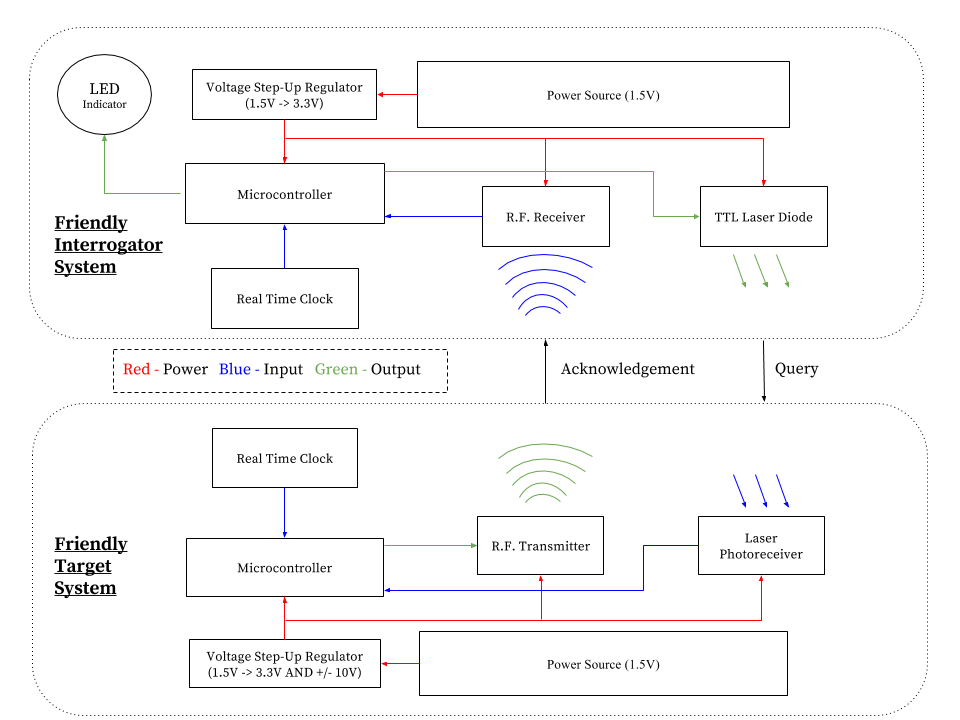
\includegraphics[scale=0.45]{System_Block_Diagram.png}
	\caption{System Block Diagram\label{fig:system-block-diagram}}
\end{figure}

The two-way communication system on both units is further divided into two one-way communication channels. The laser transmitter on board the friendly interrogator will send a signal to the photoreceivers on the friendly target. The R.F. transmitter on board the friendly target will then send acknowledgement back to the friendly interrogator. 

An important aspect of this project is encryption and ensuring an enemy cannot pose as friendly to the interrogator. This will be addressed in two ways. Both systems will contain a locally synced clock so that ...


\subsection{System Level Requirements}
Requirements are imposed on both the R.F. subsystem and the laser subsystem to accurately receive packets. From a system perspective, the requirements are as follows:\hl{Should we still keep this in?}
\begin{enumerate}
	\item R.F. Transmitter/Receiver - Must be able to both transmit and receive at least 90\% of 8-bit packets sent over a distance of 5 meters with a carrier frequency of 315 MHz ± 50 MHz.
	\item Laser Transmitter/Receiver - At least 90\% of transmitted laser packets must be received by the photoreciever at 5 m.
\end{enumerate}

Requirements are also imposed on the system speed. These are 
\begin{enumerate}
	\item Speed of System - A friendly target at 5 m should be marked friendly within 190 milliseconds.
\end{enumerate}




%SECTION - DESIGN
\section{Design}

%DESIGN PROCEDURE
\subsection{Design Procedure} 

\subsubsection{Friendly Interrogator}
\begin{figure} [H]
	\centering
	\includegraphics[scale=0.1]{interrogator_picture.png}
	\caption{Friendly Interrogator Unit\label{fig:threshold}}
\end{figure}

\hspace{5mm}\textbf{Laser Transmitter} \label{section:laser-transmitter-design-procedure}

For safety reasons, the maximum allowable power for the laser diode is $5mW$; which registers as a Class IIIa laser. The laser diode must also fall in the visible range, so that it will trigger a person's blinking reflex before eye damage occurs. Specifically, the team will use a red ($635nm$) laser. See Section \ref{section-safety-ethics} for more on safety of the laser. 

The team used a 5 mW 635 nm laser diode to transmit the unique I.D. (as specified by the 8-pin DIP switch) to the friendly target. This laser was placed inside of a casing made out of hollow aluminum tube that was created to allow the user to adjust the spot size on the laser dot. The laser can be seen in Figure \ref{fig:} The laser diode, sourced by a transistor, allows for pulsing of a unique identification number at $5kHz$. The limiting factor for the $5kHz$ requirement was the processing speed of the $MSP430$ microcontroller; between every sampling of the photoreceiver, a significant amount of processing must occur. 



 
\hspace{5mm}\textbf{Laser Safety}

 To achieve the laser beam diameter at $300 m$ associated in the proposal, a Class 3B laser would be required. In the State of Illinois, a Class 3B laser must be registered with the Division of Nuclear Safety in the Illinois Emergency Management Agency. The 3B laser would also present a significant viewing hazard; especially in an application where the laser is intended to be pointed at people. 
 
 For the reasons stated above, the team will instead use a $5mW$ visible red laser. $5mW$ visible lasers have a low chance of injuring the eye, as the blinking reflex will save a victim from permanent damage; as opposed to IR lasers which can go unnoticed for several seconds. 
 
 The following is a calculation for the nominal ocular hazard distance (NOHD) of the laser, as defined by the ANSI Standard\textsuperscript{\cite{ANSI}}.
 
 The maximum permissible exposure (MPE), as defined by the ANSI Standard \textsuperscript{\cite{ANSI}} is the highest power or energy density of a light source that is considered safe, i.e. that has a negligible probability for creating damage. This MPE for a pulsing laser is calculated as the minimum of the following three rules:
 
 \begin{enumerate}
 	\item Any single pulse in the train must not exceed the MPE for the pulse exposure time.
 	\item The exposure from any group of pulses delivered in time T must not exceed the MPE for
 	time T, where T is 0.25 seconds (from the blinking reflex), for a visible laser. 
 	\item For thermal injury, the exposure for any single pulse within a group of pulses must not
 	exceed the single-pulse MPE multiplied by a multiple-pulse correction factor
 \end{enumerate}
 
 The laser will pulse at a rate of $40 kHz$. Assuming at most a 50\% duty cycle, each pulse will be of max length $1.25*10^{-5} s$. The divergence of the beam is smallest for the longest range; a lower divergence is more restrictive in terms of safety, so this calculation uses $300m$. 
 
 At $5mW$ with a pulse width of $1.25*10^{-5}$, the power of the laser is $6.25*10^{-8} J$. 
 
 ANSI defines several constants for use in the calculation of laser safety. The relevant constant for these calculations is the constant $C_6$. This is defined as \hl{TODO: Need to format equations properly at end}
 \begin{center}
 	\large
 	$C_6 =$
 	$\frac{\theta}{1.5}$ for $1.5 \leq \theta \leq 100$\\
 	$C_6 = 1$ for $\theta < 1.5, \theta > 100$
 \end{center}
 
 Using trigonometry, the divergence angle, $\theta$, for the laser is 
 \begin{center}
 	\large
 	$Tan^{-1}(\frac{r}{300})* 1000$ $[mrad]$
 \end{center}
 
 Following the ANSI Standard \cite{ANSI}, the Rule 1 calculation is 
 \begin{center}
 	\large
 	$R_1 = 5*10^{-3} * C_6$
 \end{center}
 
 The Rule 2 calculation is
 \begin{center}
 	\large
 	$R_2 = 18 (T)^{0.75}$
 \end{center}
 
 The Rule 3 calculation is
 \begin{center}
 	\large
 	$R_3 = R1(T*f)^{0.25}$
 \end{center}
 
 The most restrictive rule defines the MPE 
 \begin{center}
 	\large
 	$MPE = min(R_1, R_2, R_3)$
 \end{center}
 
 The MPE, then, is\\
 {\large $min($}
 \begin{center}
 	\large
 	$ 5*10^{-3} * Tan^{-1}(\frac{.5}{300})* 1000$\\
 	$18 (.25)^{0.75}$ \\
 	$0.00833333 (0.25*40000)^{0.25}$
 \end{center}
 {\large $)$}
 
 This gives 
 \begin{center}
 	\large
 	$MPE = min(0.00833333, 6.36396, 0.0833333) = 0.00833333 [\frac{J}{m^2}]$
 \end{center}
 
 The NOHD is defined as (with $\theta$ in terms of $rad$, not $mrad$)
 \begin{center}
 	\large
 	$ \frac{\sqrt{\frac{4 * P}{\pi * MPE}} - 2w}{\theta}$
 \end{center}
 
 Where P is the power of the beam ($6.25*10^{-8} J$) and $w$ is the waist of the beam, $0.5mm$. This gives an NOHD of 
 \begin{center}
 	\large
 	$ \frac{\sqrt{\frac{4 * 6.25*10^{-8} }{\pi * 0.00833333}} - 2*0.0005}{Tan^{-1}(\frac{.5}{300})} = 1.25 m$
 \end{center}
 
 The team will take precautions to avoid eye contact with the laser within $1.25m$ of the source. If it is absolutely necessary to work with the laser powered on and a person within $1.25m$ of the laser, the person will be required to wear protective eye wear. 
 
 The risk of eye damage is mitigated by the fact that the laser is both visible, and not always powered on. 


\hspace{5mm}\textbf{R.F. Receiver} \label{section:rf-receiver-design-procedure}
\\ \hl{TODO}

\subsubsection{Friendly Target}


\begin{figure} [H]
	\centering
	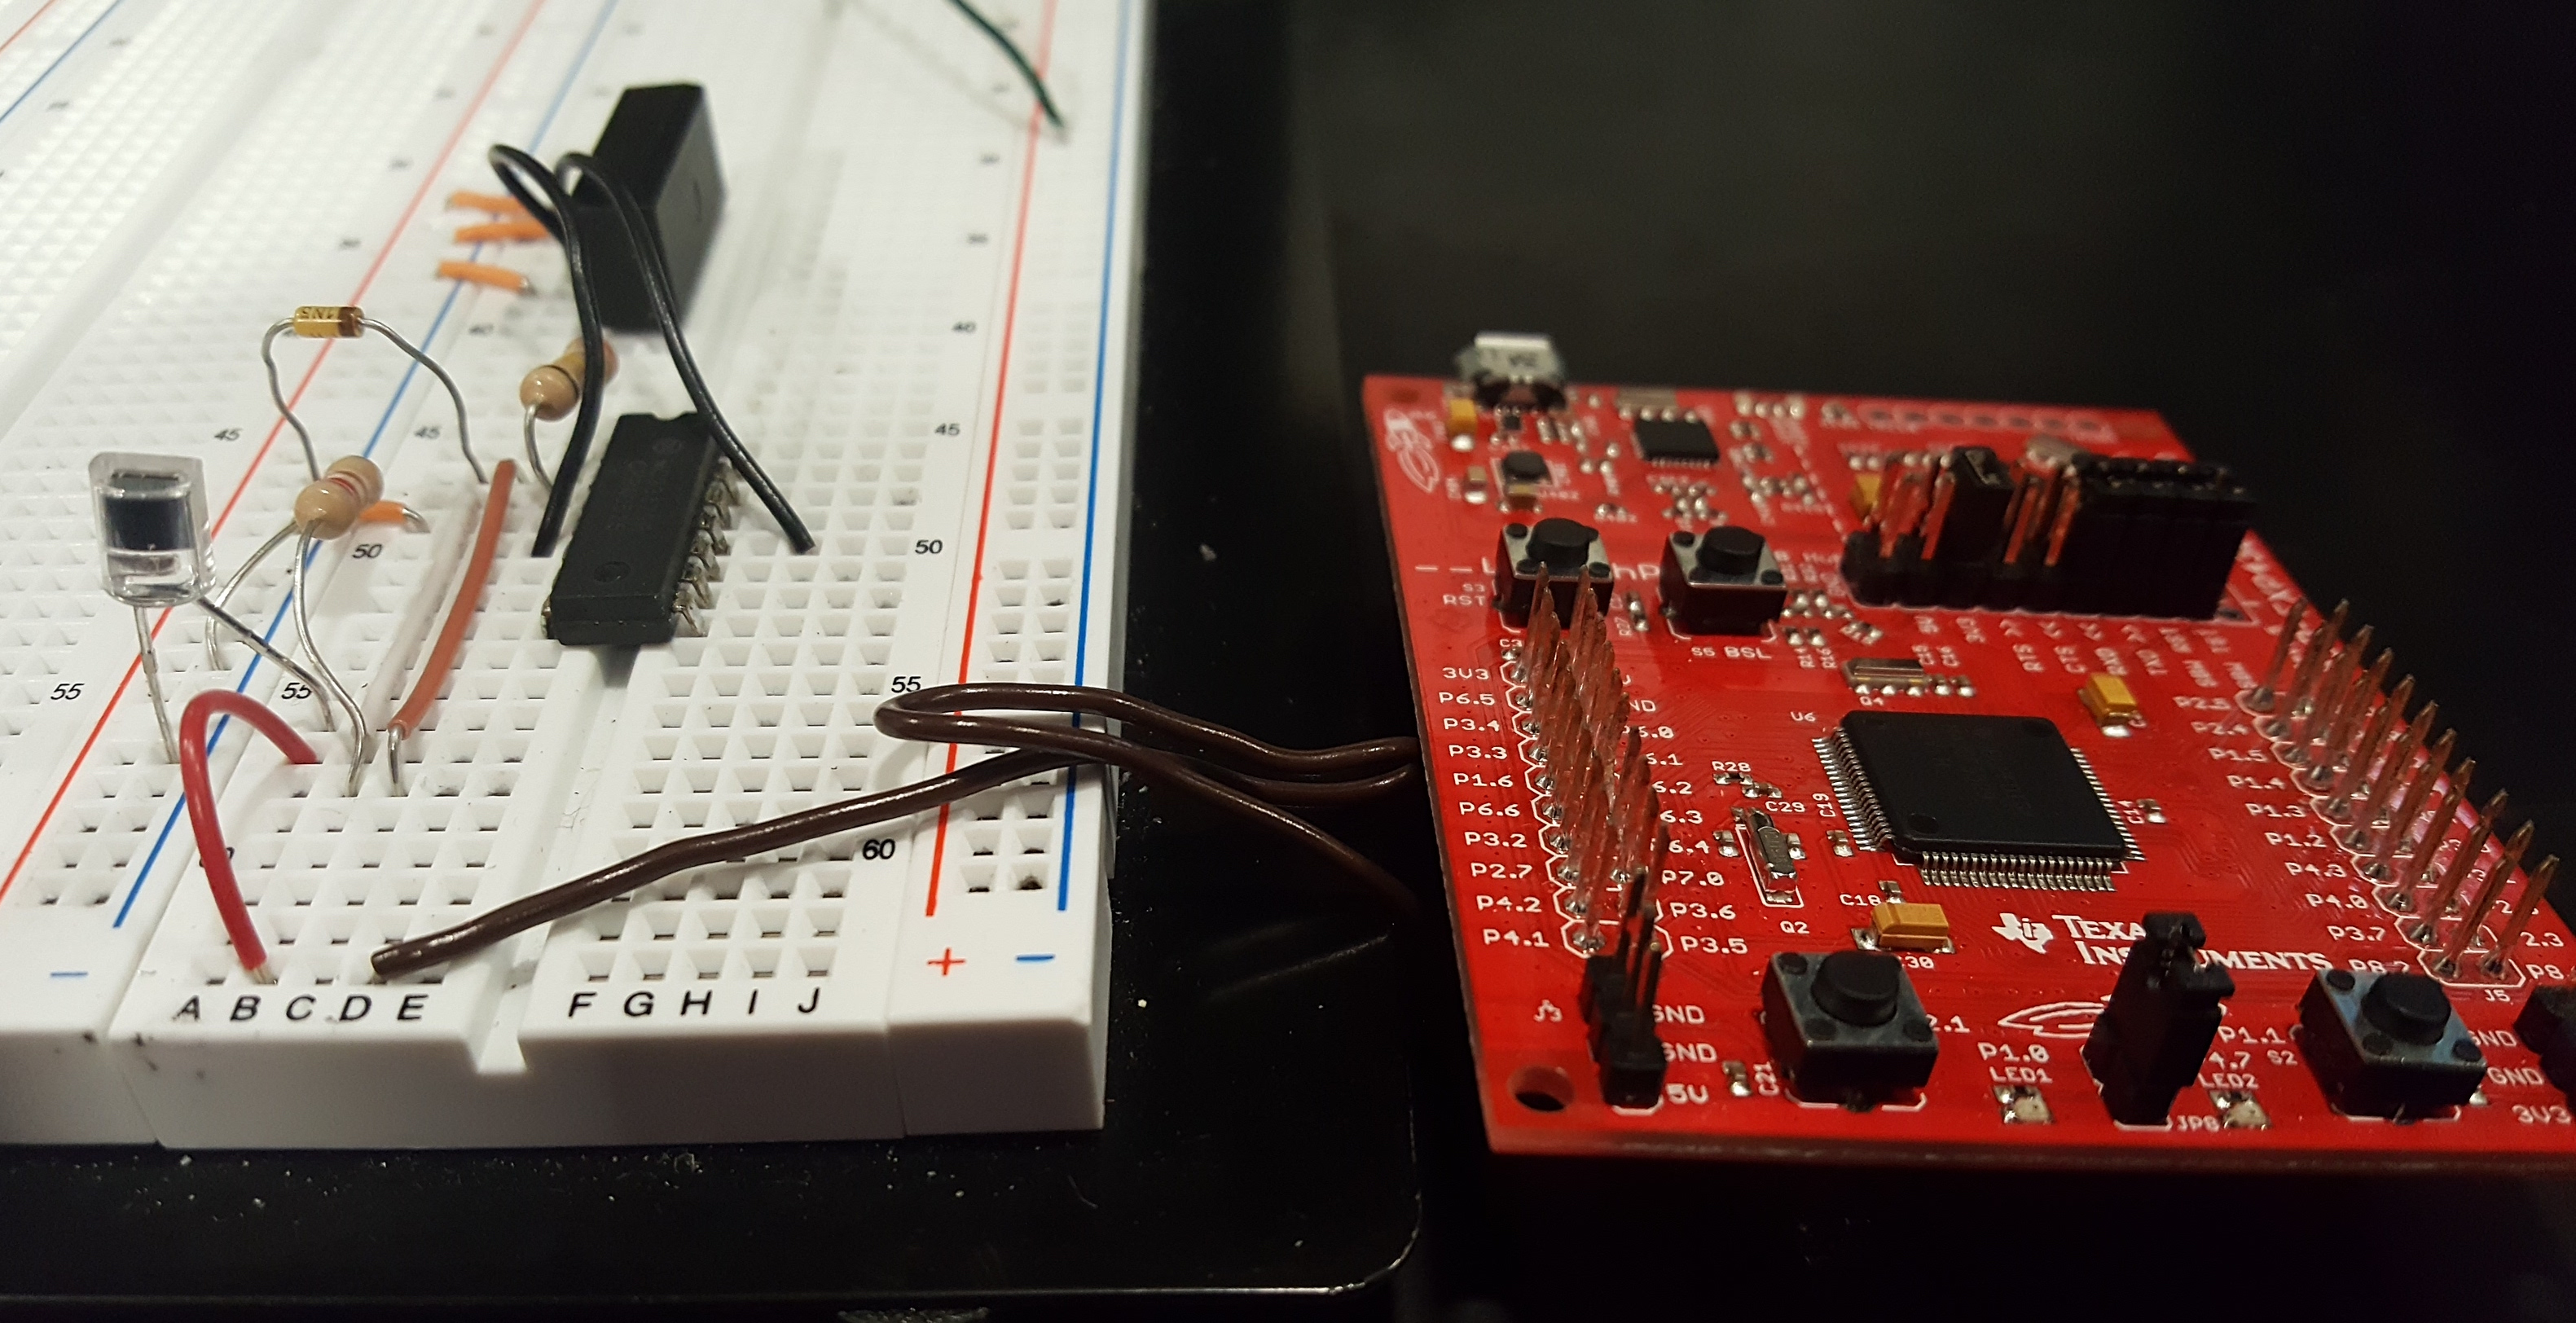
\includegraphics[scale=0.08]{target_picture.png}
	\caption{Friendly Interrogator Unit\label{fig:threshold}}
\end{figure}

\hspace{5mm}\textbf{Voltage/Power Regulation} \label{section:target-voltage-regulation-design-procedure} \\
See \ref{section:interrogator-voltage-regulation-design-procedure}

\hspace{5mm}\textbf{Laser Photoreceiver} \label{section:laser-photoreceiver-design-procedure}\\
A photodiode was chosen such that a 5kHz signal could be processed and boosted to register a value between 0 and 3.3V at a maximum distance of $30m$ from the laser source. This couples the photoreceiver requirement with the intensity of the laser diode, which is capped at $5 mW$. A detailed analysis of the choice of photodiode is in \ref{section-tolerance-analysis}



\hspace{5mm}\textbf{R.F. Transmitter} \label{section:rf-transmitter-design-procedure} \\
The requirement driving both the R.F. transmitter and receiver was the ability to broadcast and receive packets (as a pair) at the maximum distance of the project ($30m$). 
\hl{TODO: Describe some of the governing equations}


\subsubsection{System}

\hspace{5mm}\textbf{Voltage/Power Regulation} \label{section:interrogator-voltage-regulation-design-procedure}

It is required that the power stay above 3.3V for a period of 8 hours. Originally, in the design review, a 3.3V boost-converter was going to be utilized along with a single AA battery (1.5V) to supply the entire interrogator unit. This proved to be a difficult implementation to use due to the MSP drawing more power than the team expected at the time of the design review. Also, the PCB mounting of this equipment proved to be difficult for unexperienced solderers. 

For this reason, the team opted to use four AA standard alkaline batteries put through a regulator to drop the voltage supplied to the PCB down to 3.3V. In the friendly interrogator, this 3.3V output is fed directly into the MSP and R.F. modules for power. The friendly target will be explained in its respective section. 

\hspace{5mm}\textbf{Microcontroller} \label{section:system-design-procedure}\\

The microcontroller must have enough ports to service both the R.F. boards and laser/photoreceiver inputs, have enough speed to sample and decide on a packet value received at $5kHz$, and have the ability to count seconds. A vast majority of microcontrollers fit the requirements for this design, as most come with several ports, fast processors, and a built in timer.

The design decision, then, came down to ease of use and available documentation. To this end, the team chose to use the $MSP430$ series of microcontroller. Previously, the team had tried to use $MSP432s$, but these units stopped functioning mid-design. 

Other microcontroller options, including PIC and arduino were considered. Arduino was considered overkill and low difficulty for the project, PIC more difficult to work with due to less documented proprietary systems.

FROM TEMPLATE: Discuss your design decisions for each block at the most general level: What alternative approaches tothe design are possible, which was chosen, and why is it desirable? Introduce the major design equations or other design tools used; show the general form of the circuits and describe their functions.



%DESIGN DETAILS
\subsection{Design Details}


\subsubsection{Friendly Interrogator}
\hspace{5mm}\textbf{Circuit Schematics} \label{section:interrogator-circuit-schematics-design-details}
\\ \hl{TODO}

\hspace{5mm}\textbf{PCB} \label{section:interrogator-pcb-design-details}
\\ \hl{TODO}


\subsubsection{Friendly Target}
\hspace{5mm}\textbf{Circuit Schematics} \label{section:target-circuit-schematics-design-details}
\\ \hl{TODO}

\hspace{5mm}\textbf{PCB} \label{section:target-pcb-design-details}
\\ \hl{TODO}

\hspace{5mm} \textbf{Software} \label{section:target-software-design-details}\\
Incoming transmissions are broken into two parts, where a $1$ corresponds to a high at the transmission source, and a $0$ a low: 
\begin{enumerate}
	\small
	\item \textbf{Preamble} - $10101010$ 
	\item \textbf{Packet} - An 8 digit long value representing a numerical id
\end{enumerate}


Values from the photoreceiver are analog values ranging from $0-3.3V$. Because the ambient light in the room can the photoreceiver to report $0-2V$ when receiving no light from the transmitter, an algorithm was created to decide binary values of a transmission based only on the \textit{difference} between the current analog value and the analog value $200 \mu s$ before. This is similar to Non-Return to Zero Inverted (NRZI) encoding scheme widely used in many applications. This is Algorithm \ref{algo-1} shown in the appendix. Figure 

\begin{figure} [H]
	\centering
	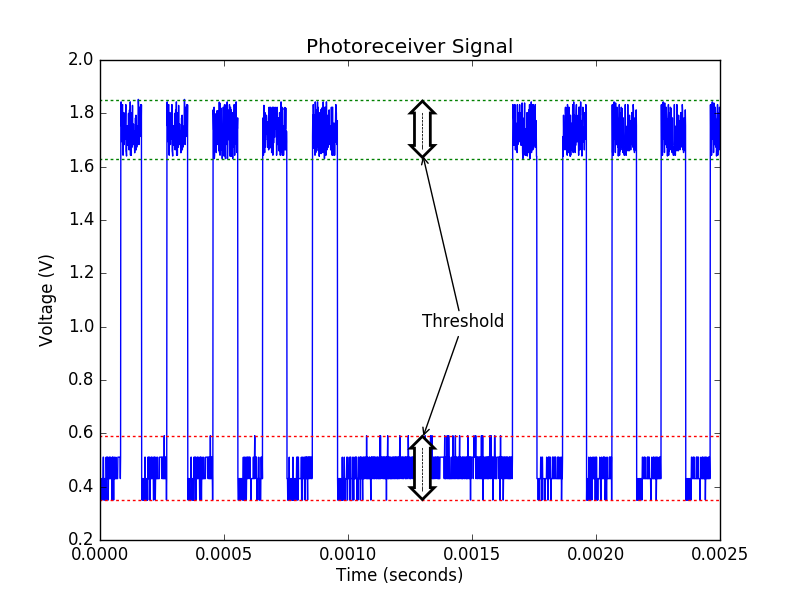
\includegraphics[scale=0.45]{threshold.png}
	\caption{Threshold Noise Difference\label{fig:threshold}}
\end{figure}


Binary values are stored in an array of length 8, since both packets and preambles are 8 bits. Because a preamble can come at any moment, an algorithm was designed both to store binary values in the array, and to always check for a preamble packet. This is Algorithm \ref{algo-2} in the appendix.

Once a preamble has been received, a simple algorithm is used to capture a packet. This is Algorithm \ref{algo-3} in the appendix. After 100 queries of a packet has received 85\% success, an acknowledgement will be sent over R.F.


Values from the photoreceiver are analog values ranging from $0-3.3V$. Because the ambient light in the room can the photoreceiver to report $0-2V$ when receiving no light from the transmitter, an algorithm was created to decide binary values of a transmission based only on the \textit{difference} between the current analog value and the analog value $200 \mu s$ before.


\makeatletter
\def\BState{\State\hskip-\ALG@thistlm}
\makeatother


Binary values are stored in an array of length 8, since both packets and preambles are 8 bits. Because a preamble can come at any moment, an algorithm was designed both to store binary values in the array, and to always check for a preamble packet 



Once a preamble has been received, a simple algorithm is used to capture a packet

\subsubsection{System}

FROM TEMPLATE: Present the detailed design, with diagrams and component values. Show how the design equations were applied. Give equations and diagrams with specific design values and data. Place large data tables in an appendix.  Circuit diagrams that are too large to be readable on a single page should be broken into pieces for presentation.  The full diagram may be included in an appendix.  Use photographs only as necessary and treat them, along with all other graphics except tables, as figures.


%SECTION - VERIFICATION
\section{Verification}

The Requirements and Verification Table is shown in the appendix.


\subsection{Laser Transmitter \& Photoreceiver}
\subsubsection{Distance Requirement}
\subsubsection{Packet Reception}
\begin{figure} [H]
	\centering
	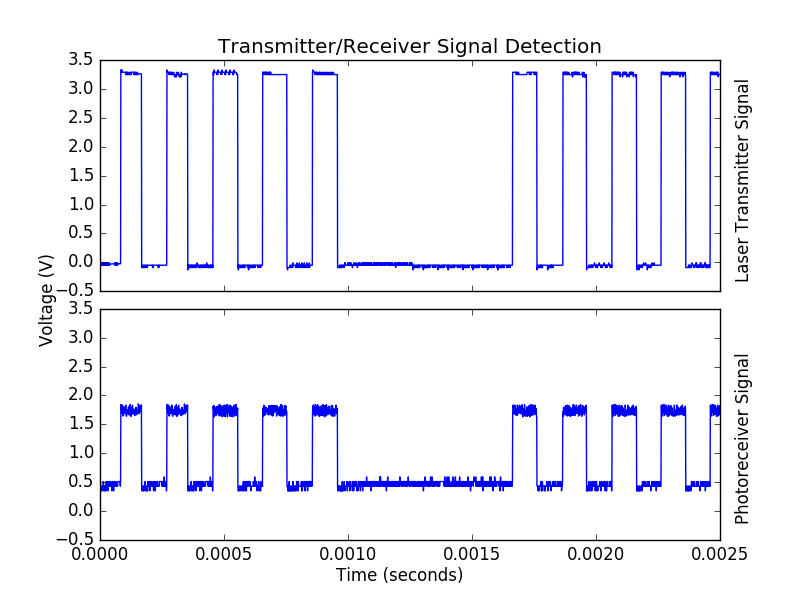
\includegraphics[scale=0.45]{packet_verification.png}
	\caption{System Block Diagram\label{fig:packet-verification}}
\end{figure}

\subsubsection {Counting Packets}
Algorithm \ref{algo-4} was used to count the number of missed packets from the photoreceiver.
The results are shown in Figure \ref{fig:transmitted-received}. The algorithm verified at 5 meters, over 85\% packet reception.

\begin{figure} [H]
	\centering
	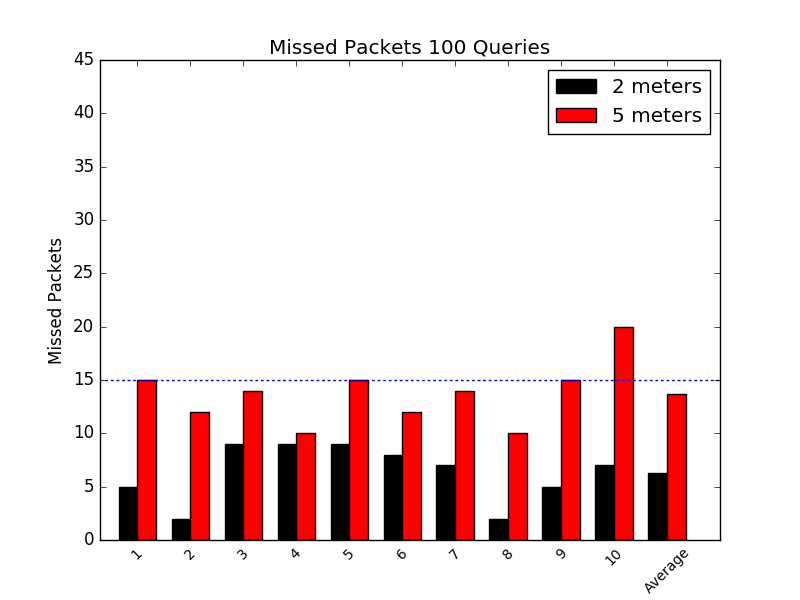
\includegraphics[scale=0.45]{transmitted_received.png}
	\caption{Missed Packets Verification\label{fig:transmitted-received}}
\end{figure}


%COSTS
\section{Costs}
\hl{TODO: Compile cost estimates}

The labor cost was calculated as follows:

\begin{center}
	Total dCost = Parts + Worker Salary (\$/hour) x 2.5 x Time (Hours) Invested In Project
\end{center}

%CONCLUSION
\section{Conclusion}
\hl{TODO}
FROM TEMPLATE: Bring together, concisely, the conclusions to be drawn. It may be appropriate, depending on the nature of the project, to begin or end with a two‐ or three‐sentence executive summary. The reader needs to be convinced that the design will work. Summarize your accomplishments. If uncertainties remain, they should be pointed out, and alternatives, such as modifying performance specifications, should be spelled out to deal with foreseeable outcomes. Use  words, not equations or diagrams. Devote a section to ethical considerations with reference to the IEEE Code of Ethics and any other applicable code (e.g., the AMA Code of Medical Ethics for certain bioengineering projects).

%REFERENCES
\section{References}
\hl{TODO}
FROM TEMPLATE: Follow the IEEE reference styles provided in this document for various kinds of sources. If you need to cite something for which there is no example, simply use common sense and provide—in a neat and orderly manner emulating the IEEE reference style—the information necessary for another researcher to find that source.   References [1]–[3] are examples of a manual, datasheet, and web page, respectively. References [4]–[7] are more standard, scholarly sources: a book, chapter in an edited book, journal article, and conference proceedings. Reference [8] is a technical report, and reference [9] is class notes. Cite all references
consecutively in the text, as is done here. (ECE Editorial Services provides a more detailed description of IEEE reference style on its wiki: http://go.illinois.edu/ecethesis .)

\clearpage
\bibliographystyle{IEEE_ECE}
% include the BibTex file here to build reference
\bibliography{Citations}\addcontentsline{toc}{section}{Reference}
\clearpage
\section*{Appendix}
\pagenumbering{gobble}

\begin{figure} [H]
	\centering
	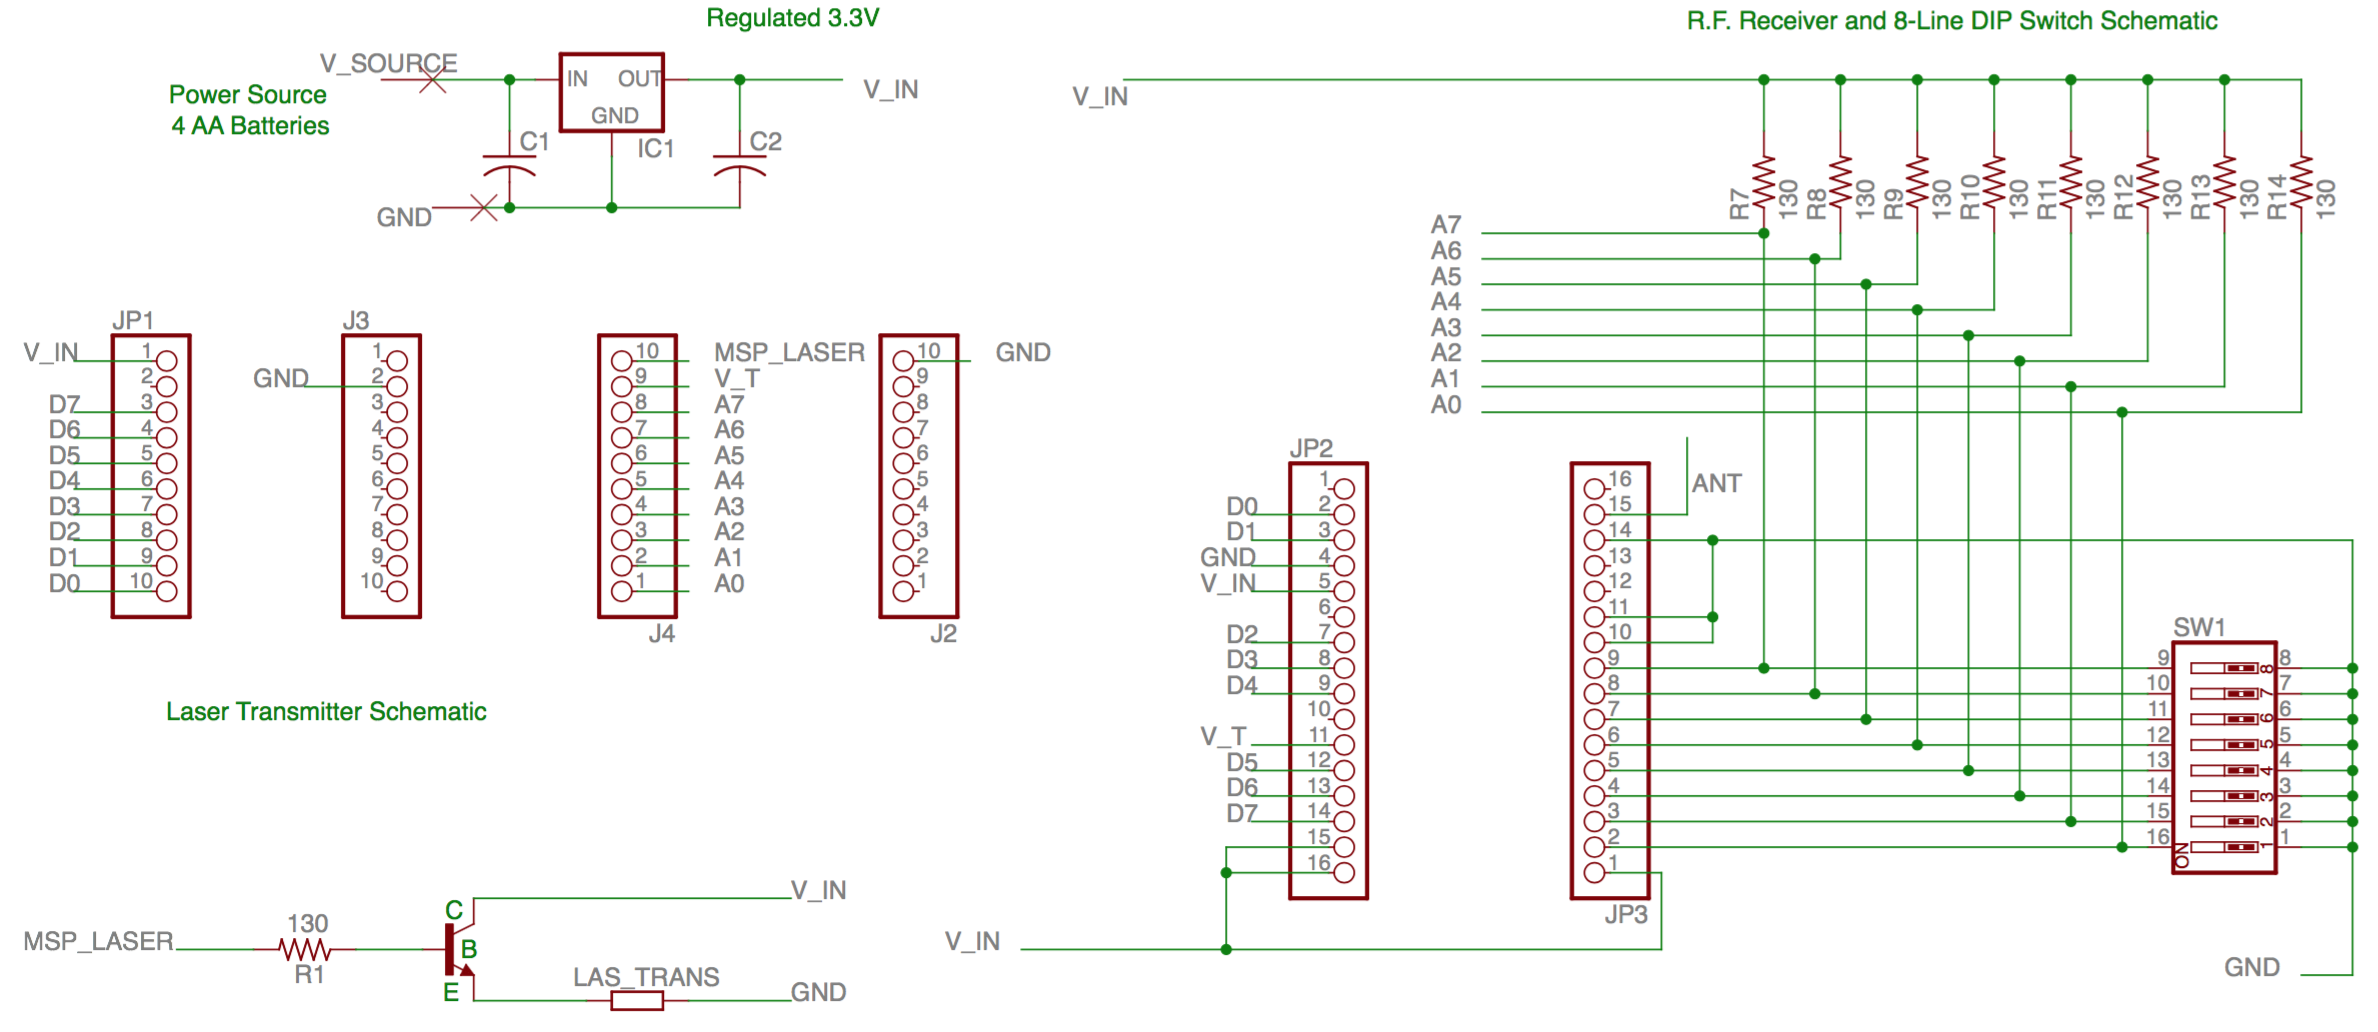
\includegraphics[scale=0.37]{friendly_interrogator_circuit.png}
	\caption{Friendly InterrogatorCircuit Schematic \label{fig:threshold}}
\end{figure}

%\begin{figure} [H]
%	\centering
%	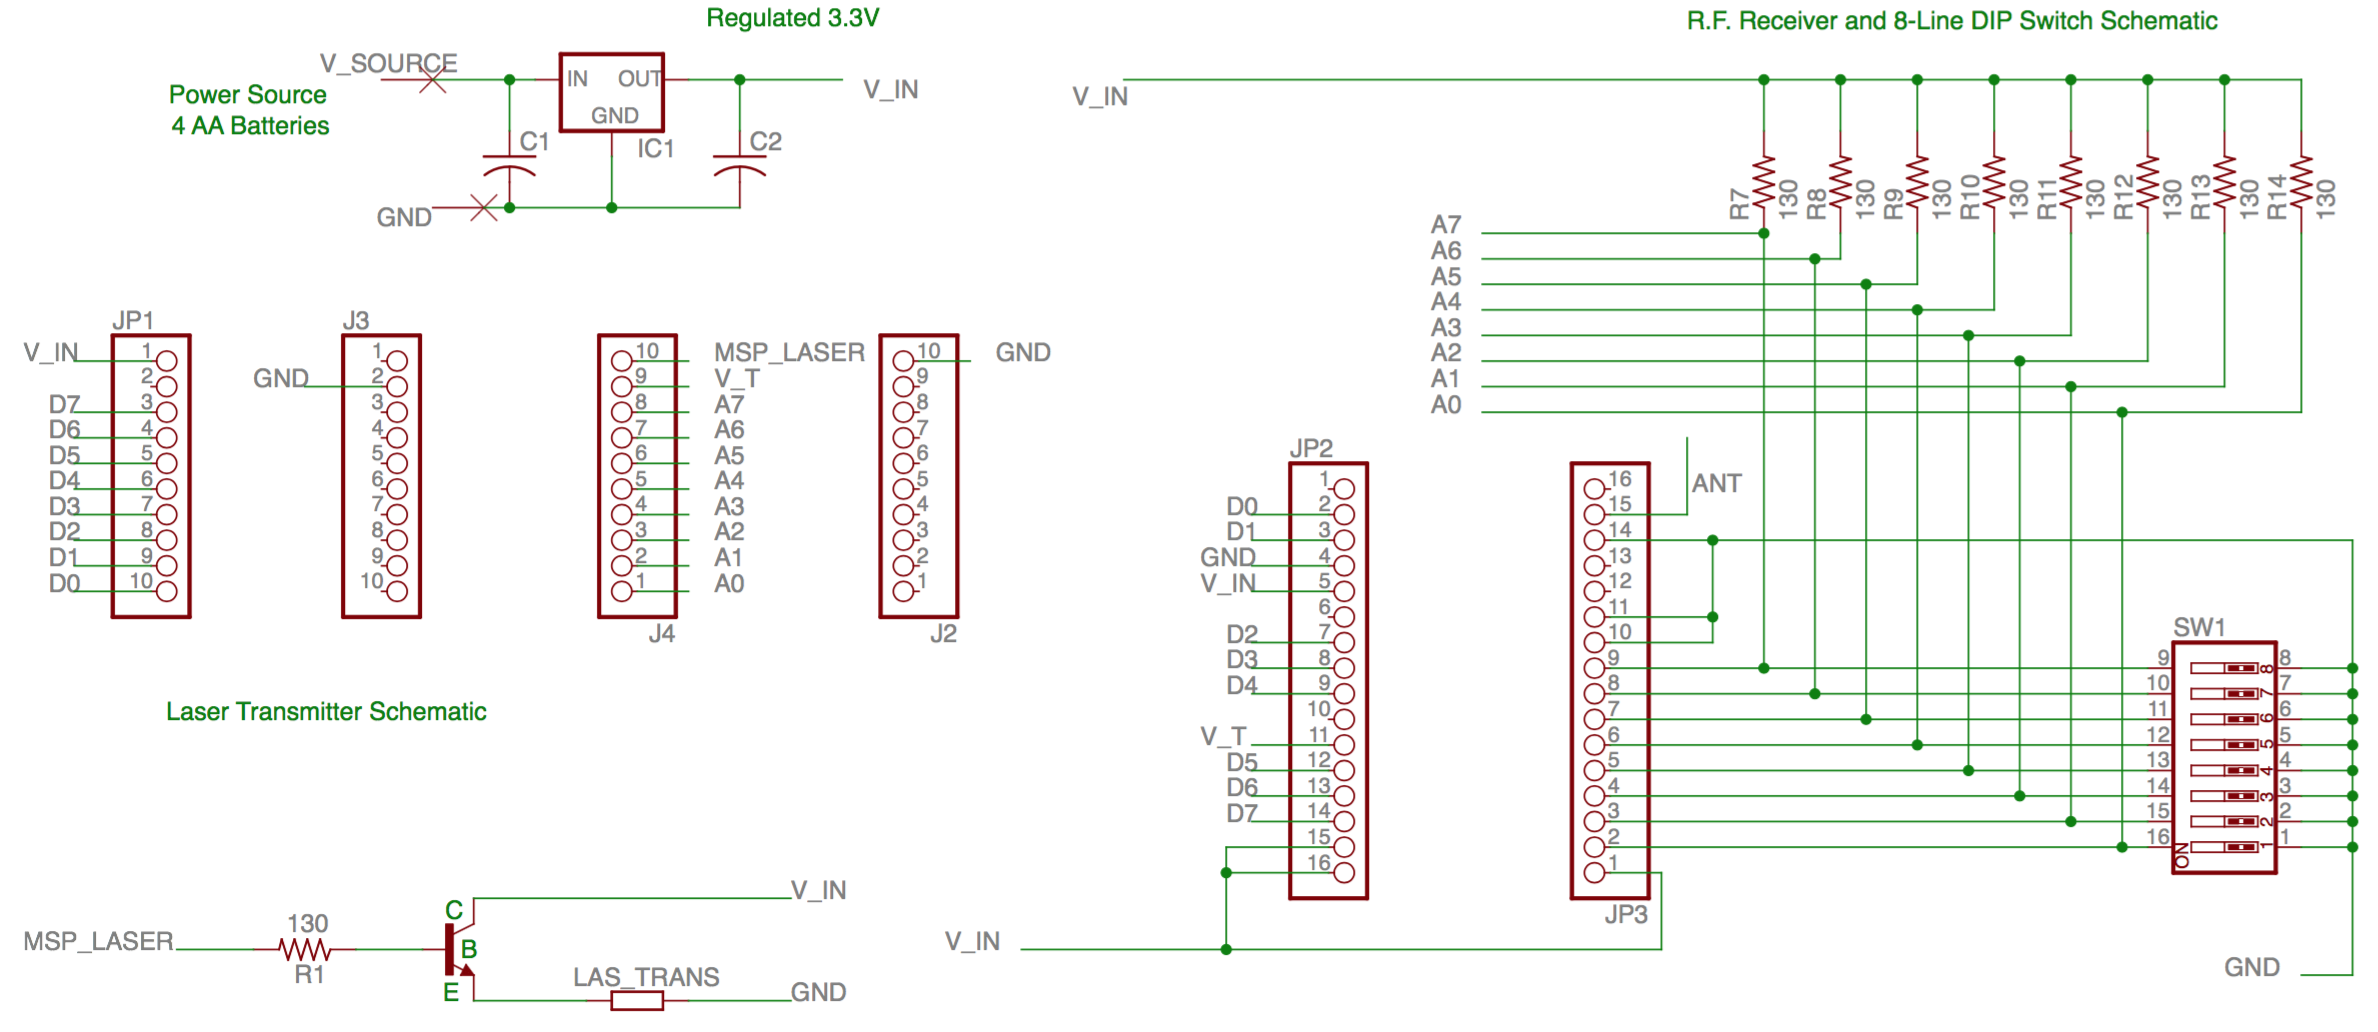
\includegraphics[scale=0.37]{friendly_interrogator_circuit.png}
%	\caption{Friendly Interrogator Circuit Schematic \label{fig:threshold}}
%\end{figure}
\hl{PUT TARGET UNIT SCHEMATIC HERE}


\makeatletter
\def\BState{\State\hskip-\ALG@thistlm}
\makeatother

\begin{algorithm}[H]
	\caption{GetCurrentBinaryValue}\label{algo-1}
	\begin{algorithmic}[1]
		\State $\textbf{Input}: \textit{currentAnalogValue},\ \textit{lastAnalogValue},\ \textit{lastBinaryValue},\ \textit{THRESHOLD}$\\
		
		\State $\textit{dif} \gets (\textit{currentAnalogValue} - \textit{lastAnalogValue})$\\\\
		
		
		//Was a 0, now a high indicates a 1
		\If {$dif > \textit{THRESHOLD}$} \\
		\quad \Return $1$\\\\
		
		//Was a 1, now a low indicates a 0
		\ElsIf {$dif < -\textit{THRESHOLD}$} \\
		\quad \Return $0$\\\\
		
		//No change from last value
		\Else\\
		\quad \Return \textit{lastBinaryValue}
		\EndIf
	\end{algorithmic}
\end{algorithm}

\begin{algorithm}[H]
	\caption{ReceivePreamble}\label{algo-2}
	\begin{algorithmic}[1]
		\State $\textit{photoBinary} \gets \text{new}\ \textit{Array}(8)$
		\State $\textit{lastBinaryValue} \gets 0$
		\State $\textit{lastAnalogValue} \gets 0$
		\State $currentIndex \gets 0$\\
		
		\State \textbf{every} $200 \mu s$ \textbf{do}\\
		\quad // Store current value\\
		\quad $\textit{currentAnalogValue} \gets \text{analogReadPhotoreceiver}$\\
		\quad $\textit{currentBinaryValue} \gets \text{GetCurrentBinaryValue}(\textit{currentAnalogValue},$\\ 
		\hspace{7.65cm} $\textit{lastAnalogValue},$\\
		\hspace{7.65cm} $\textit{lastBinaryValue})$ \\
		\quad $\text{photoBinary}[\textit{currentIndex}] \gets \textit{currentBinaryValue}$\\
		\quad $\textit{currentIndex} = (\textit{currentIndex} + 1)\ \%\ 8$\\\\
		
		\quad // Check if last 8 received values make 10101010 
		\State \quad $\textit{lastEightValues} = \text{concat}(\text{photoBinary}[\textit{currentIndex}...8],\text{photoBinary}[0..\textit{currentIndex}])$ \\
		\quad \textbf{if} $\textit{lastEightValues} == 10101010$ \textbf{then}\\
		\quad \quad ReceivePacket\\
		
		\State \quad $\textit{lastBinaryValue} \gets \textit{currentBinaryValue}$
		\State \quad $\textit{lastAnalogValue} \gets \textit{currentAnalogValue}$
		\State \textbf{end}		
	\end{algorithmic}
\end{algorithm}

\begin{algorithm}[H]
	\caption{ReceivePacket}\label{algo-3}
	\begin{algorithmic}[1]
		\State $\textit{packet} \gets \text{new}\ \textit{Array}(8)$
		\State $\textit{lastBinaryValue} \gets 0$
		\State $\textit{lastAnalogValue} \gets 0$
		\State $currentIndex \gets 0$\\
		
		\State 8 \textbf{times}, \textbf{every} $200 \mu s$ \textbf{do}\\
		\quad // Store current value\\
		\quad $\textit{currentAnalogValue} \gets \text{analogReadPhotoreceiver}$\\
		\quad $\textit{currentBinaryValue} \gets \text{GetCurrentBinaryValue}(\textit{currentAnalogValue},$\\ 
		\hspace{7.65cm} $\textit{lastAnalogValue},$\\
		\hspace{7.65cm} $\textit{lastBinaryValue})$ \\
		\quad $\text{packet}[\textit{currentIndex}] \gets \textit{currentBinaryValue}$\\
		\quad $\textit{currentIndex}\text{++}$\\\\
		
		\State \quad $\textit{lastBinaryValue} \gets \textit{currentBinaryValue}$
		\State \quad $\textit{lastAnalogValue} \gets \textit{currentAnalogValue}$
		\State \textbf{end}\\\\
		
		\Return \textit{packet}
	\end{algorithmic}
\end{algorithm}

\begin{algorithm}[H]
	\caption{CountMissedPackets}\label{algo-4}
	\begin{algorithmic}[1]
		\State \textbf{Input}: \textit{expectedPacketValue}\\
		\State $\textit{missedPackets} \gets 0$\\
		ReceivePreambleAndPacket // Get first packet to ensure transmission started
		
		\State $100.\textbf{times}\ \textbf{do}$\\
		\quad ReceivePreambleOnce // Receive next 8 bits as preamble, ignore if not a correct preamble \\
		\quad \textbf{if} ReceivePacket $\neq$ \textit{expectedPacketValue} \textbf{then} \\
		\quad \quad \textit{missedPackets}++
		\State \textbf{end}
	\end{algorithmic}
\end{algorithm}
\clearpage

\begin{figure} [H]
	\centering
	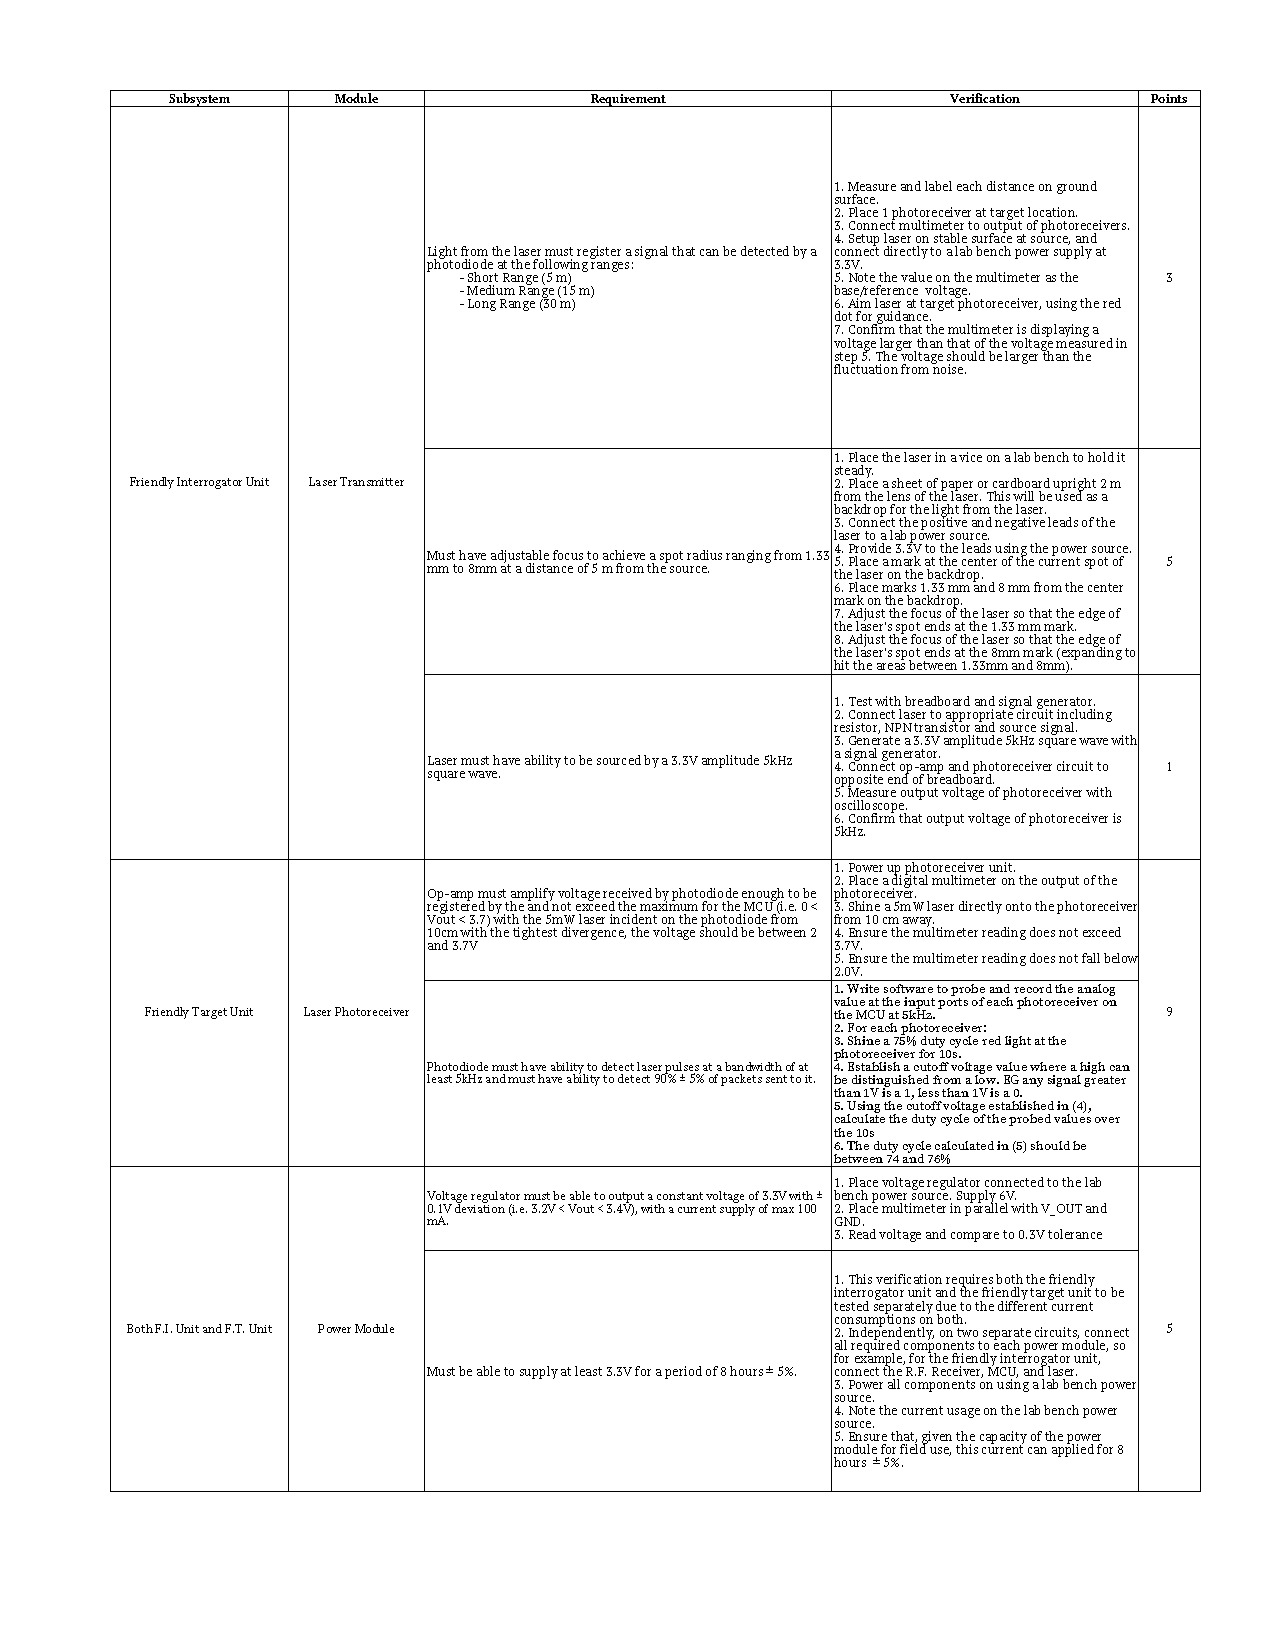
\includepdf[page=1, scale=0.85] {Requirements-Verification.pdf}
\end{figure}
\clearpage

\begin{figure} [H]
	\centering
	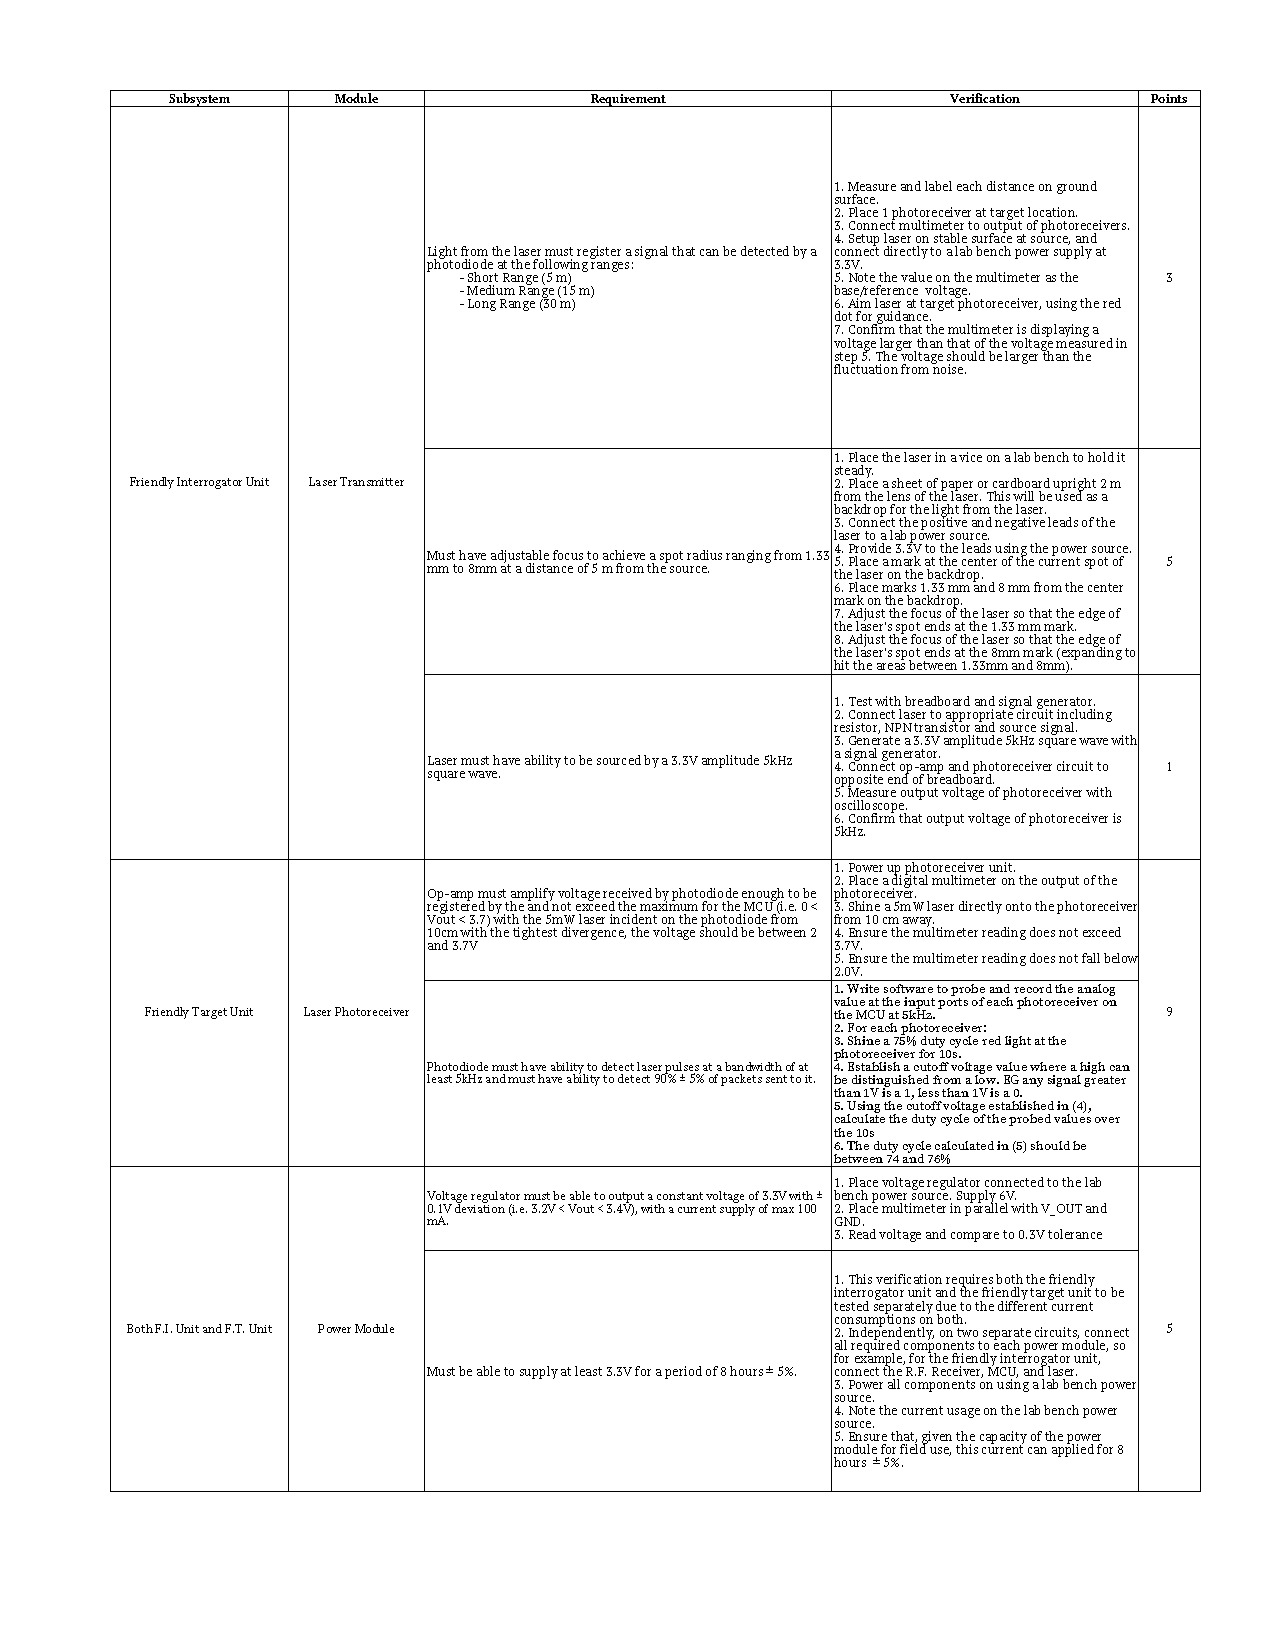
\includepdf[page=2, scale=0.85] {Requirements-Verification.pdf}
\end{figure}

\end{spacing}
\end{document}

